%%& -job-name=targetfile
\documentclass[
        oneside,      %%coloque  % no in\'icio desta linha para imprimir frente e verso 
        english,			
%	french,				
%	spanish, 
        brazil			 
        ]{configcefetmglpd}


\usepackage[T1]{fontenc}		
\usepackage[utf8]{inputenc}		%% Para converter automaticamente acentos como digitados normalmente no teclado. Mude utf8 para latin1 se precisar. 

%\usepackage{lmodern} %no caso do modelo Latex, pode-se usar a família de fontes lmodern como aqui indicado, no lugar de Arial e Times New Roman.
\usepackage{times}

\usepackage{lastpage}
\usepackage{indentfirst}		
\usepackage{color}			
\usepackage{graphicx}		
\usepackage{float}
\usepackage{svg}
\usepackage{microtype} 
\usepackage{hyperref}
\usepackage{xurl}
\usepackage{pdflscape}
\usepackage[printonlyused]{acronym}

\graphicspath{{Figuras/}} % Diretório onde estão localizadas as figuras

%% -----------------------------------------------------------------------------

%% Obs.: Alguns acentos foram omitidos.

\titulo{Título do Trabalho} %% O título do trabalho deve ser colocado dentro das chaves {}. 
\subtitulo{Subtítulo, se houver}  %% Acrescentar % no início desta linha se NÃO tiver subtítulo. Se tiver,o subtítulo do trabalho deve ser colocado dentro das chaves {}. 

\tituloIngles{Title} %% O título do trabalho em inglês deve ser colocado dentro das chaves {} .
\subtituloIngles{subtitle (se tiver)}  %% Acrescentar % no início desta linha se NÃO tiver subtítulo. Se tiver,o subtítulo em inglês do trabalho deve ser colocado dentro das chaves {}.

\autor{Nome completo} %%O nome completo do autor deve ser colocado dentro das chaves {}
\autorVirg{Sobrenome, Nome do autor} %%Acrescentar o sobrenome do autor, separado por vírgula, antes do restante do nome do autor. Ex.: Silva, José da
\autorSobrenome{Sobrenome} %% Apenas o último sobrenome dever ser acrescentado dentro das chaves
\matricula{12345678} %%Matrícula do aluno autor do trabalho

\local{Leopoldina, MG} %%Não alterar
\mesentrega{12} %%Colocar o mes da entrega dentro das chaves {}, em número. Por exemplo, 1 para janeiro; 2 para fevereiro ...
\data{2023} %%Colocar APENAS o ano da entrega dentro das chaves {}. Por exemplo, 2019.

\orientador[Orientador]{Nome do orientador} %%Colocar o nome completo do orientador(a) dentro das chaves {}. Entre os colchetes [], use [Orientador] ou [Orientadora] para identificação
\coorientador[Coorientador]{Nome do coorientador (se hover)} %%Colocar o nome completo do co-orientador(a) dentro das chaves {}. Entre os colchetes [], use [Orientador] ou [Orientadora] para identificação
\orientadorTitulo{Msc} %%Colocar a titulação do(a) orientador(a) dentro de chaves {}. Ex: Msc., Dr., Dra., etc.
\coorientadorTitulo{Msc.} %%Colocar a titulação do(a) co-orientador(a) dentro de chaves {}. Ex: Msc., Dr., Dra., etc.
\siglaInstituicaoCoorientador{CEFET-MG} %% Alterar caso o coorientado não seja do CEFET-MG

\instituicao{Centro Federal de Educação Tecnológica de Minas Gerais} %% Não alterar
\siglaInstituicao{CEFET-MG} %% Não alterar

\faculdade{Unidade Leopoldina} %% Não alterar

\programa{Engenharia de Controle e Automação} %% Não alterar
\objeto{Trabalho de Conclusão de Curso}  %% Trabalho de Conclusão de Curso - graduação ; Dissertação - mestrado
\natureza{\printaobjeto ~apresentado ao Curso de \printaprograma do \printainstituicao, do Campus Leopoldina, como parte do requisito para obtenção do título de Engenheiro de Controle e Automação.} %% Não alterar

% Data da aprovação
\aprovacaoDia{Dia} %% Colocar dentro das chaves {} o NÚMERO do dia da Data de aprovação. Ex: 15
\aprovacaoMes{Mês} %% Colocar dentro das chaves {} o mês por extenso da Data de aprovação. Ex: janeiro
\aprovacaoAno{Ano} %%  Colocar dentro das chaves {} o NÚMERO do ano da Data de aprovação. Ex: 2021

% Dados do Avaliador 1
\avaliadorUm{Nome e sobrenome} % Nome e sobrenome
\titulacaoAvaliadorUm{Titulação} % Titulação
\siglaInstituicaoAvaliadorUm{Instituição} % Sigla da institução de ensino vinculado

% Dados do Avaliador 2
\avaliadorDois{Nome e sobrenome} % Nome e sobrenome
\titulacaoAvaliadorDois{Titulação} % Titulação
\siglaInstituicaoAvaliadorDois{Instituição} % Sigla da institução de ensino vinculado

% Dados do Avaliador 3 (Se houver, apagar o "%" da frente das próximas 3 linhas)
%\avaliadorTres{Nome e sobrenome} % Nome e sobrenome
%\titulacaoAvaliadorTres{Titulação} % Titulação
%\siglaInstituicaoAvaliadorTres{Instituição} % Sigla da institução de ensino vinculado

% Dados da ficha catalográfica
\NumCatalog{AXXX} % Disponibilizado pela biblioteca
\CDU{CDU 681.5} % Número fixo para obras de eng. de controle e automação. Não alterar

%% Abaixo, prencher com os dados da parte final da ficha catalografica
\finalcatalog{1. Palavra-chave. 2. Palavra-chave. 3. Palavra-chave. I. Sobrenome, Nome do orientador Nome do meio II. Centro Federal de Educação Tecnológica de Minas Gerais. Unidade Leopoldina.} % alterar com os dados do trabalho 


% Pacotes para referência bibliográfica. Não alterar as linhas abaixo
%\usepackage[round, numbers]{natbib} % Referência númérica (não usado nesse trabalho) 
%\usepackage{natbib} % Referência utilizando o sistema autor-data
\usepackage[alf]{abntex2cite}

\begin{document}


%%---------------- Elementos Pré-textuais -----------------------------


%% Capa do Trabalho. (Não alterar)
\printacapa

%% Folha de rosto (Não alterar)
\printafolhaderosto

%% O aluno deverá solicitar a ficha na página da Biblioteca de Leopoldina. 
%% Ficha catalográfica. AO IMPRIMIR, DEIXAR NO VERSO DA FOLHA DE ROSTO. (Não alterar)
\printacatalog  


%% Folha de Aprovação. (Não alterar)
\printafolhaaprov


%% Dedicatória. ELEMENTO OPCIONAL. Caso desejar não usar, acrescentar % antes de todas as linhas até \end{dedicatoria}
 \begin{dedicatoria}
  		A dedicatória deve ser escrita com o estilo de texto “Dedicatória” e ficar no final da página. Neste local colocam-se pequenos parágrafos (não muitos) homenageando as pessoas importantes da sua trajetória acadêmica.\\  		
  		Este não é um item obrigatório do TCC \cite{bib:abnt14724}. Caso opte por não colocar dedicatória, deve-se retirar esta seção.
 \end{dedicatoria}

 
%% Agradecimentos. ELEMENTO OPCIONAL. Caso desejar não usar, acrescentar % antes de todas as linhas até \end{agradecimentos}
\begin{agradecimentos}
Os agradecimentos devem ser escritos com estilo “Corpo de texto”. O ideal é que os agradecimentos não passem de uma página. Os agradecimentos são opcionais \cite{bib:abnt14724}, porém, é altamente recomendável que faça parte do trabalho por ser um espaço para valorização das pessoas que contribuíram de alguma forma.
\end{agradecimentos}


%% Epígrafe. ELEMENTO OPCIONAL. Deve conter os dados do autor. A obra usada na epígrafe deve constar nas referências.
\begin{epigrafemais}
	“a epígrafe não é obrigatória \cite{bib:abnt14724}, portanto esta página pode ser retirada. Toda epígrafe deve estar entre aspas e no final da página.”\\
	Colocar aqui o nome do autor
\end{epigrafemais}


%% RESUMOS

%% Resumo em Português. ELEMENTO OBRIGATÓRIO.
\begin{resumo_cefetmg}
	
\aplicaresumo

Escrever o resumo do TCC. Este é um item obrigatório de acordo com a NBR 14724 \cite{bib:abnt14724}. 
Quanto a sua extensão os resumos devem ter de 150 a 500 palavras. 
A elaboração deste resumo deve seguir a NBR 6028 \cite{bib:abnt6028}. 
O texto do resumo deve estar em parágrafo único. Todas as palavras devem estar com letras minúsculas com exceção dos substantivos
próprios e nomes científicos, separadas por ponto e vírgula. 
As palavras-chave são inseridas abaixo do resumo com uma linha de 1,5 em branco separando-as.

\begin{center}
\textbf{Palavras-chave}: gestação; cuidado pré-natal; Aedes Aegypti; IBGE; Brasil.
\end{center}

\end{resumo_cefetmg}
 
 
%% Resumo em Inglês. Opcional, mas recomndável.
\begin{abstract_cefetmg}
 \begin{otherlanguage*}{english}

\aplicaabstract

Escrever a tradução do resumo do TCC. Uma das vantagens de se ter o abstract no TCC é que, quando alguém fizer uma busca na
internet por palavras-chaves em inglês, seu trabalho terá mais chances de ser encontrado. 

\begin{center}
\textbf{Keywords:} Palavra 1. Palavra2. Palavra 3. %Finalizadas por ponto e aplicaializadas por letra maiuscula.
\end{center}
  \end{otherlanguage*}
\end{abstract_cefetmg}


\printatermo

%% Lista de ilustrações.Sao consideradas ilustrações: desenhos, esquemas, fluxogramas, figuras, fotografias, gr\'aficos, mapas, organogramas, plantas, quadros, entre outros. Tabelas não são consideradas ilustrações.

\pdfbookmark[0]{\listfigurename}{lof}

%Caso as ilustrações do trabalho sejam todas do mesmo tipo (por exemplo, todas do tipo organograma), coloque % no início das duas linhas abaixo. 
\figvariadas   %Use este comando somente caso as ilustrações não sejam todas do mesmo tipo. 
\listfigvariadas  %Use este comando somente caso as ilustrações não sejam todas do mesmo tipo e caso queira inserir a lista delas. 

%\listoffigures*  %Use este comando quando todas as ilustrações são do mesmo tipo e caso queira inserir a lista delas. Em geral, se mantém comentado

\cleardoublepage

\pdfbookmark[0]{\listtablename}{lot}

%% Lista de tabelas. Se NÃO houver tabela nenhuma, colocar % na frente da linha debaixo.
\listoftables*   

\cleardoublepage


%% Lista de abreviaturas e siglas. Não deve haver sinal grafico entre as siglas e abreviaturas e o significado. 

\begin{siglas} %%ALTERAR OS EXEMPLOS ABAIXO, CONFORME A NECESSIDADE
	\acro{EX}{Example}
	\acro{HiRDLS}{High-Resolution Dynamics Limb Sounder}
	\acro{MLS}{Microwave Limb Sounder}
	\acro{TES}{Tropospheric Emission Sounder}
 
%  Deve obedecer a ordem alfabética. A sigla, quando mencionada pela primeira vez no texto, deve ser indicada entre parênteses, precedida do nome completo (ABNT 14724, 2011). Exemplo: Interface Homem Máquina (IHM).
  \end{siglas}


%% Lista de símbolos. Nao deve haver sinal grafico entre o simbolo e o seu significado.
\begin{simbolos} %%ALTERAR OS EXEMPLOS ABAIXO, CONFORME A NECESSIDADE
  \item[$ \forall $] Para todo
  \item[$ \in $] Pertence
  
%  Observação: Em trabalhos cuja formulação matemática requerer um número muito grande de símbolos e variáveis (geralmente letras gregas), sugere-se a colocação de uma seção de lista de símbolos. Devem obedecer a ordem com que aparecem no texto.
 \end{simbolos}

 
%% Sumário. Não alterar
\pdfbookmark[0]{\contentsname}{toc}
\tableofcontents*
\cleardoublepage

%% ------------------- Elementos Textuais -------------------------

\textual %Não alterar


\chapter{Introdução ao Modelo} %% Título do Capítulo dentro das chaves {}
\label{cap:introducao_modelo} %% Palavra chave para referência cruzada no texto. SUGERE-SE colocar ser "cap:" como demostrado no modelo para melhor organização em textos maiores

Este modelo deve ser seguido com extrema obediência às recomendações para que todos os TCCs mantenham a mesma formatação. A aplicaiativa de utilizar o modelo é para criar um padrão de qualidade na apresentação gráfica dos TCCs. O \LaTeX é um sistema de preparação de documentos que utiliza linhas de comando e visa facilitar a formatação de textos científicos ou livros. Sugere-se utilizar o software "TeXstudio", pois esse modelo foi realizado nessa plataforma, além de ser gratuito e de código aberto. % Novo parágrafo é só acrescentar dois "ENTER"'s do teclado

As formatações do texto estão todas configuradas previamente, portanto, NÃO se deve alterar o arquivo "configcefetmglpd.cls". Qualquer alteração, mínima que seja, pode fazer com que não se compile corretamente o documento.

Nos itens a seguir serão apresentadas as dicas e formas de utilização deste modelo.

Este modelo prevê a impressão em anverso (somente frente). Não poderá haver impressão em anverso e verso (frente e verso). A única folha impressa em verso deve ser a de ficha catalográfica, que deve estar no verso da primeira folha.


\section{Estrutura do Modelo} %% Título da seção dentro das chaves {}
\label{sec:estrutura_modelo}  %% Palavra chave para referência cruzada no texto. SUGERE-SE colocar ser "sec:" como demostrado no modelo para melhor organização em textos maiores
O modelo conta com a parte pré-textual (folha de rosto até sumário), que é contada e não numerada \cite{bib:abnt6027}. As partes textual e pós-textual são numeradas com algarismos arábicos. A numeração de páginas prossegue da parte pré-textual.

A parte textual geralmente conta com um capítulo de introdução, alguns capítulos de desenvolvimento e um capítulo de conclusão. O número de capítulos de cada trabalho é definido entre o orientador e o estudante. Neste modelo serão colocados oito Capítulos, pois, raramente um trabalho conta com tantas seções e é mais fácil adequá-lo as necessidades do estudante, bastando retirar os capítulos excedentes (apagar o capítulo excedente e a quebra de seção abaixo do mesmo).\ac{EX} \ac{MLS}

A parte pós-textual conta com bibliografia, apêndices e anexos. A bibliografia contará com um capítulo especial explicando como deve ser feita. Os apêndices são partes do trabalho desenvolvidas pelo aluno, mas que não ficariam adequadas ao desenvolvimento do texto, por este motivo, merecem uma citação no texto indicando que se encontram no apêndice. Os anexos são documentos que complementam as informações da parte textual, mas não são de autoria do estudante, por exemplo datasheets de componentes.

Este modelo conta com uma estrutura de tópicos que gera o sumário automaticamente. Nesta estrutura existem vários níveis, que são associados a “estilos de texto”. Estes estilos de texto serão mostrados na seção \ref{sec:estilo_de_texto}. %referência cruzada

\section{Exemplos de Níveis das Seções (Este é o Segundo Nível)} %% Título da seção dentro das chaves {}
\label{sec:exemplos_niveis_secao}
A seguir estão os exemplos de subseções dos quais podem ser copiadas as propriedades utilizando-se o pincel de formatação. 
Todos os cinco níveis das seções devem constar no sumário de acordo com a NBR 6027 \cite{bib:abnt6024}.

\subsection{Exemplo de Terceiro Nível} %% Título da subseção dentro das chaves {}
Corpo do texto

\subsubsection{Exemplo de Quarto Nível} %% Título da subsubseção dentro das chaves {}
Corpo do texto

\subsubsubsection{Exemplo de Quinto Nível} %% Título da subsubsubseção dentro das chaves {}
Corpo do texto

\subsubsection{Exemplo de Quarto Nível}
Corpo do texto

\subsubsubsection{Exemplo de Quinto Nível}
Corpo do texto corpo do texto corpo do texto corpo do texto corpo do texto corpo do texto.

\section{Alíneas e Subalíneas} \label{sec:alineas_subalineas}
As alíneas são subdivisões de uma seção ou subseção. Elas são precedidas por letras minúsculas e parêntese. 
As alíneas abaixo estão no estilo de texto “Alínea” e servem como base para terem suas características copiadas com o pincel de 
formatação do Word. As alíneas devem ser conforme a seguir \cite{bib:abnt6024}:

%Exemplo para Alíneas
\begin{enumerate}[label=\alph*)]
	\item os diversos assuntos que não possuam título próprio, dentro de uma mesma seção, devem ser subdivididos em alíneas; 
	\item o texto que antecede as alíneas termina em dois pontos; 
	\item as alíneas devem ser indicadas alfabeticamente, em letra minúscula, seguida de parêntese. Utilizam-se letras dobradas, quando esgotadas as letras do alfabeto;
	\item as letras indicativas das alíneas devem apresentar recuo em relação à margem esquerda;
	\item o texto da alínea deve começar por letra minúscula e terminar em ponto-e-vírgula, exceto a última alínea que termina em ponto final;
	\item o texto da alínea deve terminar em dois pontos, se houver subalínea;
	\item a segunda e as seguintes linhas do texto da alínea começam sob a primeira letra do texto da própria alínea.
\end{enumerate}

Do mesmo modo, as subalíneas devem ser conforme as alíneas a seguir:

%Exemplo para Alíneas e Subalíneas
\begin{enumerate}[label=\alph*)]
	\item as subalíneas devem começar por travessão seguido de espaço:
	\begin{itemize}
		\item[$-$] este é um exemplo de subalínea;
		\item[$-$] este é um exemplo de subalínea;
	\end{itemize}
	\item as subalíneas devem apresentar recuo em relação à alínea;
	\item o texto da subalínea deve começar por letra minúscula e terminar em ponto-e-vírgula. A última subalínea deve terminar em ponto final, se não houver alínea subsequente;
	\item a segunda e as seguintes linhas do texto da subalínea começam sob a primeira letra do texto da própria subalínea \cite{bib:abnt6024};
	\begin{itemize}
		\item[$-$] este é um exemplo de subalínea;
		\item[$-$] este é um exemplo de subalínea;
	\end{itemize}
\end{enumerate}

\section{Espaçamentos}

De acordo com o Manual de Normalização de Trabalhos Acadêmicos do CEFET-MG (MANUAL CEFET, 2023), todo o texto deve ser 
digitado com a seguinte: parágrafo justificado, sem hifenização, entre linhas com espaçamento de 1,5 ponto e recuo de primeira 
linha de 1,25cm. Citações de mais de três linhas, notas de rodapé, referências, legendas das ilustrações e 
das tabelas e a natureza do trabalho (tipo, objetivo, nome da instituição a que é submetido e área de concentração) devem ser 
digitados com espaçamento simples. Quanto às referências, ao final do trabalho, estas devem estar separadas entre si por um espaço 
simples em branco e alinhadas à esquerda. Além disso, devem ser elaboradas conforme a ABNT NBR 6023 (última atualização em 2020) 
\cite{bib:abnt6023}.

Todos os estilos utilizados neste modelo possuem seus espaçamentos definidos no momento da sua criação e não devem, 
em hipótese alguma, serem alterados.

\section{Páginal Virada na Posição Paisagem} 
Deve-se evitar colocar páginas na posição paisagem, mas se for inevitável, esta deve ser colocada em uma seção individual. Quando for necessário o uso de página virada é só utilizar o código a seguir.

%Exemplo para utilizar página no formato paisagem
\begin{landscape}
Esta página está virada porque pretende-se colocar lado a lado os objetivos e os métodos utilizados para alcançar estes objetivos.
\end{landscape}

\chapter{Figuras, Tabelas, Equações e Notas de Rodapé} \label{cap:fig_tab_eq}
Os textos técnicos geralmente são enriquecidos com figuras, tabelas e equações. Todas as figuras e tabelas utilizadas deverão ser comentadas no texto. Mesmo que se julgue que a figura seja autoexplicativa, não se deve deixar margem para erros de interpretação, daí a necessidade de textos explicativos. As próximas subseções trarão uma explicação de como usar figuras, tabelas e equações e irá trazer informações de como fazer referências cruzadas entre legendas de figuras e tabelas e referências no texto.

\section{Como Utilizar Figuras no TCC} \label{sec:figuras_tcc}
A Figura \ref{fig:1figs} foi colocada utilizando a função \textit{minipage}. A fonte é obrigatória mesmo que seja do próprio autor, conforme determina a NBR 14724 \cite{bib:abnt14724}.

A numeração da legenda é automática. Quando a figura for citada no texto deve-se utilizar a função \textit{ref}. Por exemplo, o texto “Figura \ref{fig:1figs}” do início da Seção \ref{sec:figuras_tcc} foi inserido automaticamente ao usar a função citada.

%Exemplo de como usar Subfiguras
\begin{figure}[h]
	\larguratexto{14cm}
	\centering
	\caption{Técnicas de levitação magnética. a) eletromagnética (EML), b) eletrodinâmica (EDL) e c) supercondutora (SML).}%
	\begin{minipage}[t]{3cm}%
		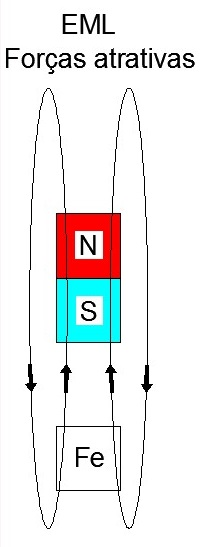
\includegraphics[width=3cm]{cap3_1.jpg}
		\par \centering a)
		\label{fig:EML}
	\end{minipage}%
	\hspace{1cm}
	\begin{minipage}[t]{6cm}%
		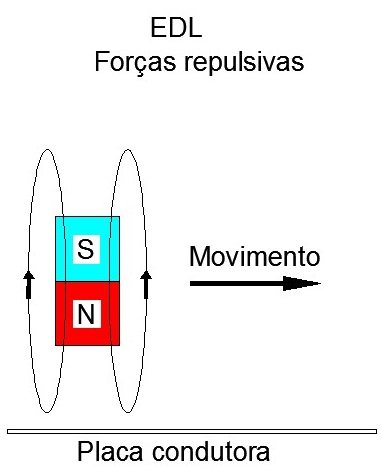
\includegraphics[width=6cm]{cap3_2.jpg}
		\par \centering b)
		\label{fig:EDL}
	\end{minipage}%
	\hspace{1cm}
\begin{minipage}[t]{3cm}%
	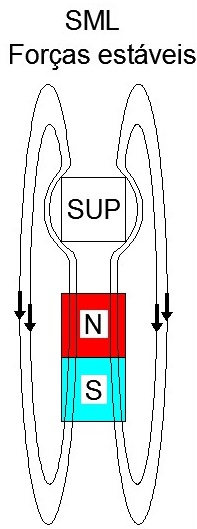
\includegraphics[width=3cm]{cap3_3.jpg}
	\par \centering c)
	\label{fig:SML}
\end{minipage}%
	\fonte{\cite{bib:mattos}}
	\label{fig:1figs}%
\end{figure}

\section{Como Utilizar Tabelas no TCC}
O procedimento para utilização de tabelas e referências cruzadas é o mesmo do de figuras. A diferença é que a legenda fica acima da tabela. A Tabela \ref{tab:lista_Mag} pode ser copiada e colada em outras partes do texto e depois alterada de acordo com a necessidade.

O ideal é que a tabela caiba em uma única folha, mas se o tamanho da tabela obrigar a utilização de mais de uma folha, o cabeçalho deve ser repetido.

%Exemplo de como usar uma tabela
\begin{table}[!h]
	\normalsize
	\caption{Lista das vinte e duas conferências MagLev ocorridas até hoje.}
	\label{tab:lista_Mag}
	\begin{center}
		%\setlength{\tabcolsep}{8pt}
		\begin{tabular}{ l | c | l | c | l}
			\hline
			Conferência Maglev & Ano & Cidade & Continente & Veículo/Protótipo apresentado\\ \hline
			1st & 1977 & Boston, USA & America &  \\
			2nd & 1978 & Miyazaki, Japan & Asia & ML-500 \\
			3rd & 1979 & Hamburg, Germany & Europe & TR-05 \\
		\end{tabular}
	\end{center}
	\fonte{\cite{bib:mattos}}
\end{table}

\section{Como Utilizar Equações no TCC}

As equações também ficam dentro de tabelas, assim como as figuras. A Equação (\ref{eq:equacao1}) utilizando a função \textit{equation}.  Quando se desejar fazer referência cruzada deve-se proceder da mesma forma que no referenciamento de figuras. O exemplo é a equação (\ref{eq:equacao1}).

%Exemplo de como usar equações
\begin{equation}
	\label{eq:equacao1}
	\alpha = \frac{F_1 + F_2 - P_1' - P_2'}{M_1+M_2} = \frac{F_1 + F_2}{M_1 + M_2}-g.sen(\alpha)
\end{equation}

\section{Como Utilizar Notas de Rodapé}
Quando pretende-se dar algum tipo de explicação de algo que foi colocado no texto, mas, essa explicação é longa ou não é muito relevante para o entendimento, ela pode ser colocada como nota de rodapé. Outra aplicação é no caso de informações que não são necessárias para o entendimento do texto, mas o autor acha enriquecedor colocar informações adicionais.

No fragmento de texto, a seguir, pretende-se dar uma explicação sobre as leis de Kepler e dar o nome completo de quem formulou as leis. Essas informações podem não ser necessárias para todos os leitores. Neste caso o leitor continuaria lendo o texto sem interrupções, mas caso alguém tenha a curiosidade de se informar mais a respeito, pode recorrer à nota de rodapé para isso. Outro exemplo é a palavra “heliocentrismo”, nem todo mundo sabe do que se trata, por isso, o autor resolveu colocar uma nota de rodapé.

“... Ao demonstrar a consistência que havia entre o sistema por si idealizado e as leis de Kepler\footnote{As leis de Kepler são as três leis do movimento planetário definidas por Johannes Kepler (1571 – 1630), um matemático e astrônomo alemão. Essas leis foram a principal contribuição de Kepler à astronomia e à astrofísica.}  do movimento dos planetas, foi o primeiro a demonstrar que os movimentos de objetos, tanto na Terra como em outros corpos celestes, são governados pelo mesmo conjunto de leis naturais. O poder unificador e profético de suas leis era centrado na revolução científica, no avanço do heliocentrismo\footnote{Em astronomia, heliocentrismo é a teoria que coloca o Sol, em sua apresentação aplicaial, estacionário no centro do universo; ou em sentido estrito, situado aproximadamente no centro do sistema solar, no caso do heliocentrismo renascentista}  e na difundida noção de que a investigação racional pode revelar o funcionamento mais intrínseco ...” %Exemmplo com notas de rodapé

\section{Considerações Parciais}
A figura, a tabela e a equação foram referenciadas no texto com a utilização de referências cruzadas. O Capítulo \ref{cap:ref_cruzadas} irá descrever a importância da utilização desta forma de referenciar.

As notas de rodapé são sinalizadas no texto com um número sobrescrito e as notas contendo as explicações vem no final da página. As marcações e as notas sempre aparecem na mesma página .

\chapter{Referências Cruzadas} \label{cap:ref_cruzadas}
As figuras, tabelas e equações possuem numeração vinculada ao capítulo, por exemplo, a Figura \ref{fig:lajes_concreto} é a primeira figura do capítulo três. Caso esta figura seja mudada de um capítulo para outro a numeração será atualizada automaticamente. O mesmo acontece se um capítulo for introduzido ou retirado antes deste.

Em um trabalho de TCC é comum que capítulos inteiros sejam remanejados para melhorar a cronologia do trabalho, então, as numerações automáticas e o referenciamento cruzado é fundamental para poupar trabalho e evitar erros na numeração.

%Exemplo de declarar figuras
\begin{figure}[h]
	\larguratexto{12cm}  %Mesma largura da ilustração, dada em "[width=12cm]" abaixo
	\caption{Lajes de concreto e detalhes da montagem dos ímãs.}
	\label{fig:lajes_concreto}
	\begin{center}
		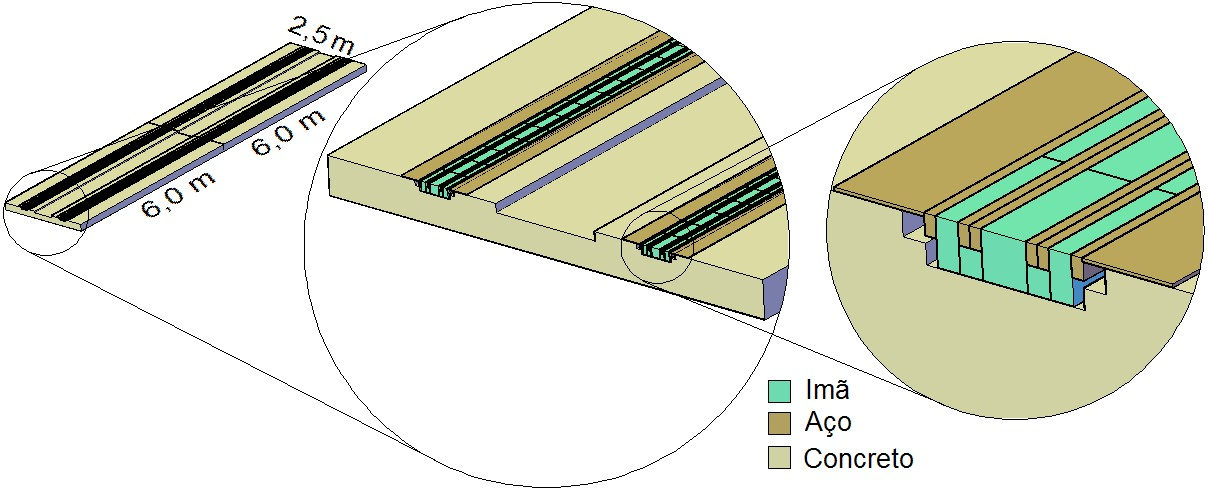
\includegraphics[width=12cm]{cap4_1.jpg}
		\fonte{\cite{bib:mattos}} %%Indicar a fonte consultada (elemento obrigat\'orio, mesmo que seja produ\c{c}\~ao do pr\'oprio autor).
	\end{center}
\end{figure}

\section{Referenciamento Cruzado de Equações}
Figuras e tabelas devem, obrigatoriamente, serem citadas e explicadas no corpo do texto. Mas, quando se trata de equações, existem duas formas de referenciar. A primeira é igual a de figuras e tabelas e a segunda é coloca-las em forma de texto corrido. As Seções \ref{subsec:refer_eq_texto_corrido} e \ref{subsec:eq_ref_numero} mostram os exemplos das duas formas de apresentação das equações no texto. Preferencialmente deve-se usar a forma apresentada na Seção \ref{subsec:refer_eq_texto_corrido}, por se tratar de uma maneira mais formal e adotada em grande parte dos livros técnicos.

\subsection{Exemplo de Referenciamento de Equações em Texto Corrido} \label{subsec:refer_eq_texto_corrido}
Segue exemplo de referenciamento em texto corrido. É possível notar que a pontuação é colocada considerando as equações como parte do texto.

(...) De acordo com a equação (3.6) (Obs.: citando equação de outro ponto do texto fictício), a máxima aceleração possível para o veículo totalmente carregado é de 0,3 m/s$^2$, isso resulta em uma aceleração de aproximadamente 0,03 g, que é menor que qualquer um dos valores da (3.1). Mas se no plano de operação do MagLev for determinado que o veículo só poderá operar nas condições de carregamento AW0 e AW1, as acelerações máximas possíveis mudarão para,

\begin{equation}
	\label{eq:Aw0}
^	a_{AW0} = \frac{\textit{Força~máxima~dos~motores}}{\textit{Massa~do~veículo~descarregado}} = \frac{1800N}{AW0/g}
	=\frac{1800N}{21.000N/g}=0,086g
\end{equation}

e

\begin{equation}
	\label{eq:Aw1}
	a_{AW1} = \frac{\textit{Força~máxima~dos~motores}}{\textit{Massa~do~veículo~descarregado}} = \frac{1800N}{AW1/g}
	=\frac{1800N}{31.680N/g}=0,056g
\end{equation}

Em ambas as condições as acelerações normais e de emergência não foram ultrapassadas. Falta verificar a componente vertical. Para o pior caso, a aceleração vertical é dada por:

\begin{equation}
	\label{eq:Avert}
	a_{Vert} = a_{AW0}.sen(\theta)=0,086g.sen(0,61^o)=0,001g
\end{equation}

Onde: $a_{Vert}$ é a aceleração vertical e $\theta$ é o ângulo de inclinação da via.

Após todas as verificações conclui-se que o MagLev sempre irá operar em condições confortáveis de aceleração. (...)

\subsection{Exemplo de Referenciamento de Equações pelo Número} \label{subsec:eq_ref_numero}

(...) De acordo com a equação (3.6) (Obs.: citando equação de outro ponto do texto fictício), a máxima aceleração possível para o veículo totalmente carregado é de 0,3 m/s$^2$, isso resulta em uma aceleração de aproximadamente 0,03 g, que é menor que qualquer um dos valores da (3.1). Mas se no plano de operação do MagLev for determinado que o veículo só poderá operar nas condições de carregamento AW0 e AW1, as acelerações máximas possíveis são as mostradas nas Equações (\ref{eq:Aw0_2}) e (\ref{eq:Aw1_2}).

\begin{equation}
	\label{eq:Aw0_2}
	a_{AW0} = \frac{\textit{Força~máxima~dos~motores}}{\textit{Massa~do~veículo~descarregado}} = \frac{1800N}{AW0/g}
	=\frac{1800N}{21.000N/g}=0,086g
\end{equation}

e

\begin{equation}
	\label{eq:Aw1_2}
	a_{AW1} = \frac{\textit{Força~máxima~dos~motores}}{\textit{Massa~do~veículo~descarregado}} = \frac{1800N}{AW1/g}
	=\frac{1800N}{31.680N/g}=0,056g
\end{equation}

Em ambas as condições as acelerações normais e de emergência não foram ultrapassadas. Falta verificar a componente vertical. Para o pior caso, a aceleração vertical é dada pela Equação (\ref{eq:Avert_2}).

\begin{equation}
	\label{eq:Avert_2}
	a_{Vert} = a_{AW0}.sen(\theta)=0,086g.sen(0,61^o)=0,001g
\end{equation}

Onde: $a_{Vert}$ é a aceleração vertical e $\theta$ é o ângulo de inclinação da via.

Após todas as verificações conclui-se que o MagLev sempre irá operar em condições confortáveis de aceleração. (...)

\section{Considerações Parciais}
Deve-se sempre utilizar referências cruzadas, mas se por algum motivo optar-se pela numeração manual o texto deve ser totalmente revisto a cada inserção de nova legenda e os índices de figuras e tabelas deverão ser criados manualmente e atualizados constantemente. Em resumo, fatalmente algo ficará errado.

\chapter{Como Gerenciar Fontes Bibliográficas}
A pesquisa bibliográfica é fundamental para criar a base técnica e científica do TCC. Mas, faz-se necessário creditar aos autores a propriedade intelectual. Existem diversas formas e regras para a citação de autores. No Brasil adota-se a NBR 10520 \cite{bib:abnt10520} e a NBR 6023 \cite{bib:abnt6023}.

\section{Textos de Referências Bibliográficas}
Como o próprio nome já diz, os textos pesquisados servem como referência para que o aluno de TCC escreva seu próprio texto. Copiar textos ou fragmentos de texto, traduzir literalmente, escrever “com outras palavras”, etc. Configuram plágio e são sujeitos a sansões da lei. Só é permitido copiar fragmentos de texto quando se pretende tecer comentários ou esclarecimentos sobre o texto original, para isso o fragmento deve estar entre aspas e o autor deve ser citado.

Todos os artigos, livros, revistas, anais de congresso, etc. Que deram suporte ao autor do TCC, devem ser citados no texto e constar na lista de referências após o capítulo de conclusão.

\section{Maneiras de Referenciamento}
Existem programas disponíveis para download, como o JabRef, que faz o gerenciamento das bibliografias do trabalho de uma forma facilitada. Na internet existem tutorias para esses gerenciadores que utilizam o sistema BibTex. Esses gerenciadores não foram testados com a classe atual do modelo.

Há a possibilidade de fazer esse gerenciamento no próprio arquivo de edição usando a função "bibitem", como está sendo realizado nesse modelo. A função $\cite{}$ permite chamar a referência no texto.

\section{Citações Diretas}
Para casos de citações diretas a formatação é diferente e utiliza a função abaixo.

%Exemplo de citação direta
\begin{citacao}
	As cita\c{c}\~oes diretas, no texto, com mais de tr\^es linhas, devem ser destacadas 
	com recuo de 4 cm da margem esquerda, com letra menor que a do texto utilizado 
	e sem as aspas. [...] Para enfatizar trechos da cita\c{c}\~ao, deve-se destac\'a-los indicando esta 
	altera\c{c}\~ao com express\~ao grifo nosso entre par\^enteses, ap\'os a chamada da cita\c{c}\~ao, ou grifo 
	do autor, caso o destaque j\'a fa\c{c}a parte da obra consultada. (ASSOCIA\c{C}\~AO BRASILEIRA DE NORMAS 
	T\'ECNICAS, 2002, p. 2-3)
\end{citacao}


\chapter{Instruções para Capa e Lombada}
Este capítulo foi introduzido ao modelo com a finalidade de padronizar as lombadas e capas dos TCCs produzidos no CEFET-MG, 
unidade Leopoldina.

\section{Lombada}
A capa possui alguns elementos obrigatórios e deve seguir a ordem estabelecida na norma NBR 14724 \cite{bib:abnt14724}. 
A lombada segue a norma NBR 12225 \cite{bib:abnt1225}, da seguinte forma: o título deve ser impresso no mesmo sentido do(s) 
nome(s) do(s) autor(es), abreviado, quando necessário; o título de lombada deve estar na descendente e impresso longitudinalmente 
e legível do alto para o pé da lombada. Esta forma possibilita a leitura, quando o documento está com a face dianteira voltada 
para cima (Figura 6.1). As medidas mostradas na figura devem ser seguidas exatamente como aparecem na figura, pois, quando as 
monografias forem colocadas lado a lado em uma estante de biblioteca, haverá um alinhamento correto dos elementos gráficos da
lombada.

\section{Capa}
A Capa mostrada na Figura 6.1 possui todos os elementos obrigatórios estabelecidos pelas normas NBR 14724 \cite{bib:abnt14724}. 
A capa deve obedecer exatamente o que é mostrado na figura, essa padronização busca trazer qualidade e boa apresentação visual das monografias produzidas pelos estudantes do CEFET-MG, unidade Leopoldina.

\begin{figure}[h]
	\larguratexto{15cm}  %Mesma largura da ilustração, dada em "[width=12cm]" abaixo
	\caption{Lombada e capa.}
	\label{fig:lombada}
	\begin{center}
		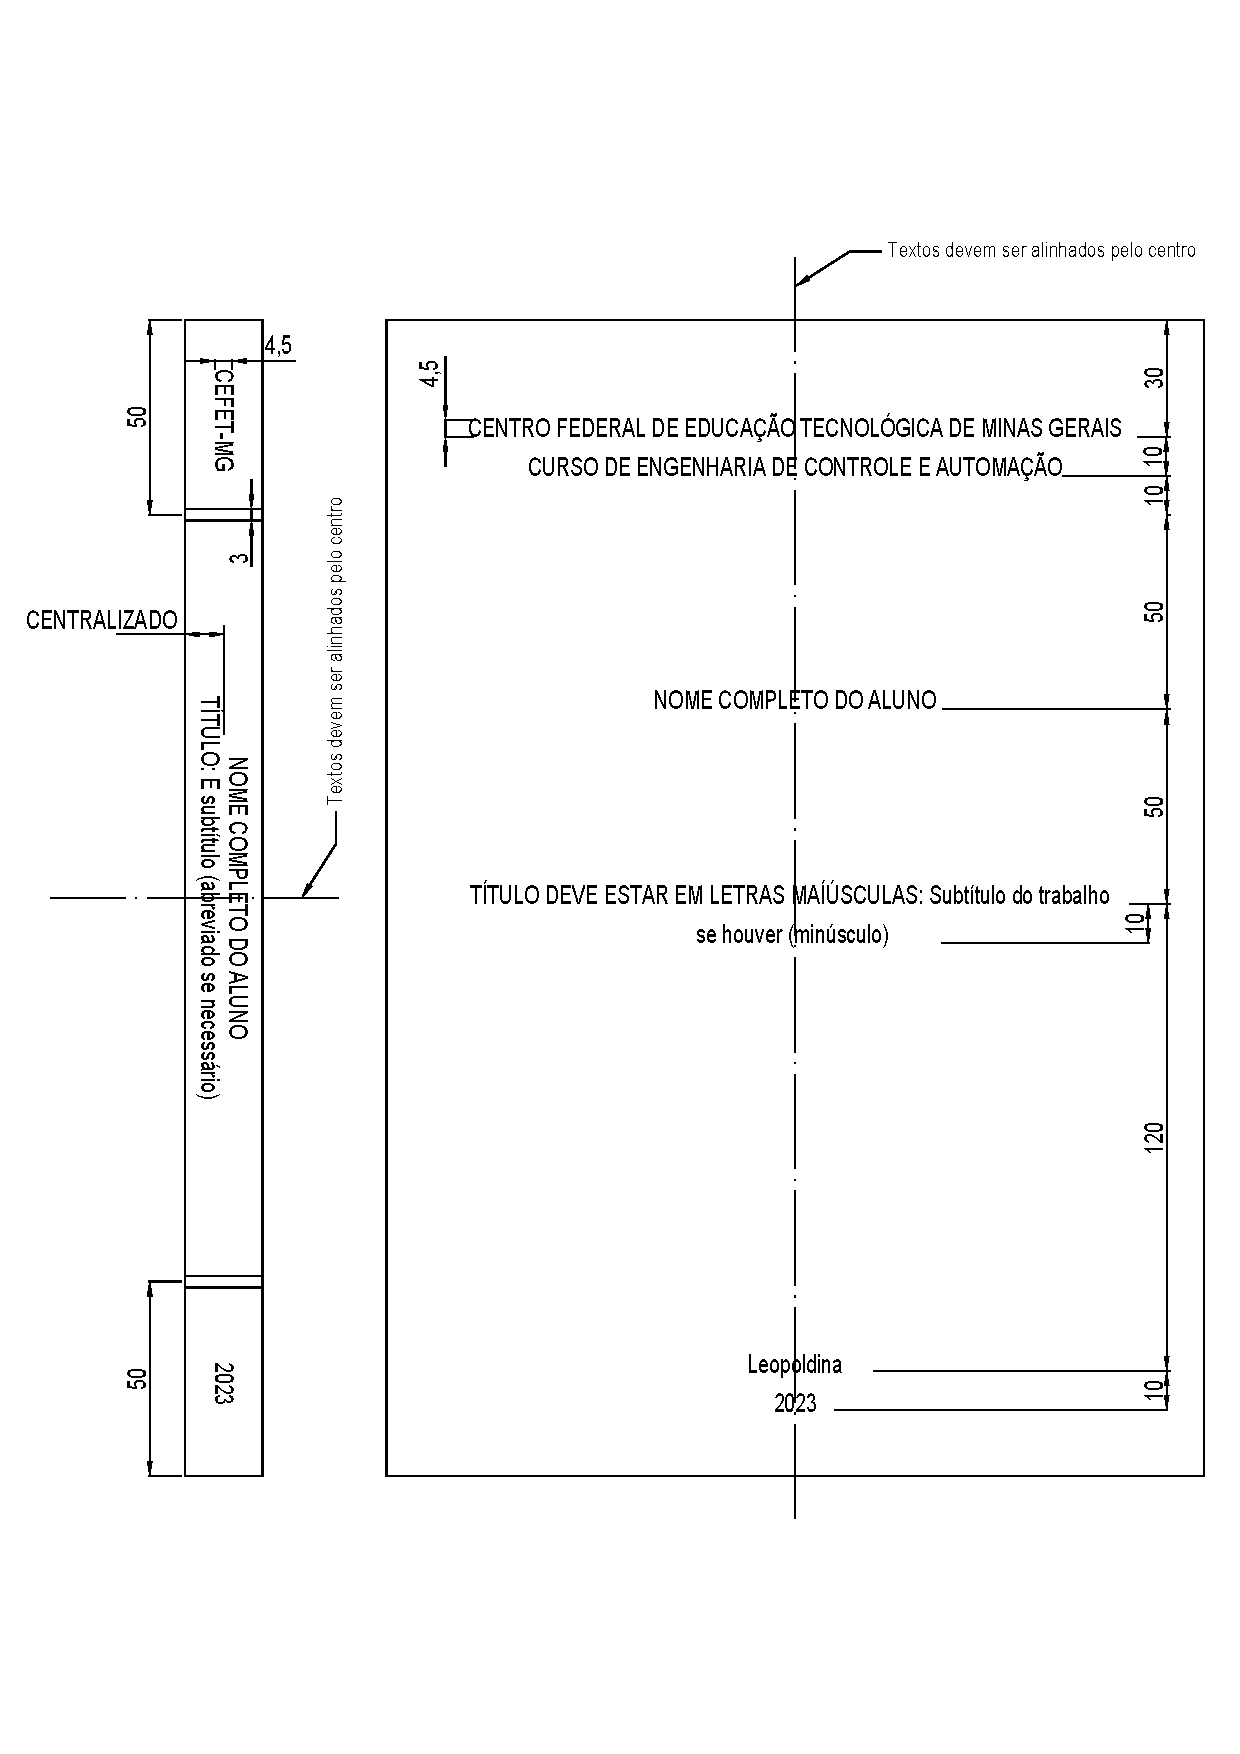
\includegraphics[width=15cm]{lombada.pdf}
		\fonte{do autor. Todas as medidas estão em milímetros.} %%Indicar a fonte consultada (elemento obrigat\'orio, mesmo que seja produ\c{c}\~ao do pr\'oprio autor).
	\end{center}
\end{figure}

\chapter{Conclusões e Trabalhos Futuros}

Neste capítulo, são apresentadas as conclusões, as considerações sobre o trabalho desenvolvido e, também, são discutidas propostas para trabalhos futuros.

\section{Conclusões}
A utilização deste modelo visa padronizar a parte editorial dos trabalhos de conclusão de curso (TCC). Os orientadores darão mais dicas além das colocadas neste documento, principalmente no tocante ao conteúdo e sequência de apresentação.

\section{Trabalhos Futuros}
Colocar aqui sugestões de trabalhos futuros.

%% -----------Elementos  Pós-Textuais --------------

\postextual 

\bibliography{referencias.bib}



%% Apendices
\begin{apendices}

\chapter{\apendseq O Primeiro Apêndice Deve Ser Colocado Aqui} 
%%Digita-se o titulo do apendice mantendo-se, antes, o comando \apendseq, como indicado.

O apêndice deve ser colocado aqui


\chapter{\apendseq O Segundo Apêndice Deve Ser Colocado Aqui} 
%%Digita-se o titulo do apendice mantendo-se, antes, o comando \apendseq, como indicado.

O apêndice deve ser colocado aqui 


\chapter{\apendseq O Terceiro Apêndice Deve Ser Colocado Aqui} 
%%Digita-se o titulo do apendice mantendo-se, antes, o comando \apendseq, como indicado.

O apêndice deve ser colocado aqui 


\end{apendices}


%% Anexos
\begin{anexos}

\chapter{\anexoseq O Primeiro Anexo Deve ser Colocado a Seguir} 
%%Digita-se o titulo do anexo mantendo-se, antes, o comando \anexoseq, como indicado.

Corpo do texto



\chapter{\anexoseq O Segundo Anexo Deve ser Colocado a Seguir} 
%%Digita-se o titulo do anexo mantendo-se, antes, o comando \anexoseq, como indicado.

Corpo do texto
  
\end{anexos}


%%% ---
\end{document}
